\documentclass[12pt]{article}
\usepackage[pdftex]{graphicx}
\usepackage{amsfonts}
\usepackage[italian]{babel}
\usepackage{graphicx}
\usepackage{color}
\usepackage{multirow,bigdelim}

\definecolor{grey}{rgb}{0.3,0.3,0.3}

\usepackage{listings, framed}
\lstset{
  language=Java,
  showstringspaces=false,
  columns=flexible,
  basicstyle={\small\ttfamily},
  frame=none,
  numbers=none,
  keywordstyle=\bfseries\color{grey},
  commentstyle=\itshape\color{red},
  identifierstyle=\color{black},
  stringstyle=\color{blue},
  numberstyle={\ttfamily},
%  breaklines=true,
  breakatwhitespace=true,
  tabsize=3,
  escapechar=|
}

%****************enlarge layout
\textheight     243.5mm
\topmargin      -20.0mm
\textwidth      480pt
\hoffset        -80pt
%*****************theorems and such
\newcounter{esnu}
\newenvironment{esercizio}{\medskip \noindent {\bf Esercizio\addtocounter{esnu}{1} \arabic{esnu}}}{}
\pagestyle{empty}
\newcommand{\liff}{\mathrel{\leftrightarrow}}   % Logical IFF Symbol
\newcommand{\metaiff}{\Longleftrightarrow}      %iff in metatheory

\begin{document}

%\begin{tabular}{llclcr}
% \hspace{-35pt} &{\bf COGNOME:} & \hspace{100pt}        &{\bf NOME:}    & \hspace{100pt}        &{\bf MATRICOLA:}%\hspace{35pt} \\
%\hline
%\end{tabular}
\begin{center} {\bf Esame di Programmazione II, 24 giugno 2019}\end{center}
%\`

\emph{
Si crei un progetto Eclipse e, nella directory dei sorgenti,
si crei il package \texttt{it.univr.tictactoe}. Si copi al suo interno
le classi del compito.
Se si realizzano nuove classi, le si crei dentro
il package \texttt{it.univr.tictactoe}.
Non si modifichi le dichiarazioni dei metodi. Si possono definire altri campi,
metodi, costruttori e classi, ma devono essere \texttt{private}.
La consegna fornita compila.
Anche la soluzione che verr\`a consegnata dovr\`a compilare,
altrimenti non verr\`a corretta.
}
\mbox{}\\

Il gioco del tris consiste in una tabella 3x3 in cui due giocatori,
alternativamente, piazzano i simboli croce e cerchio.
Vince il giocatore che per primo piazza tre simboli uguali nella
stessa riga, colonna o diagonale, come ad esempio la croce in questa immagine:
%
\begin{center}

\includegraphics[width=2.2cm]{tictactoe_wins.png}
\end{center}
%
Il gioco pu\`o anche finire in
parit\`a se tutte le caselle sono piene ma nessun giocatore ha vinto,
come nell'immagine seguente:
%
\begin{center}

\includegraphics[width=3cm]{tictactoe_draw.png}
\end{center}

\begin{esercizio}~\textbf{[14 punti]}
  Si completi la classe \texttt{TicTacToe.java}, che implementa un gioco
  del tris, dove indicato con \texttt{TODO}. Tale codice definisce gi\`a le
  variabili d'istanza \texttt{crossPlayer} e \texttt{circlePlayer}, che sono
  i due giocatori che si alternano al gioco. La loro classe \texttt{Player.java}
  \`e gi\`a scritta e completa. Si faccia attenzione a lanciare le
  eccezioni come indicato nei commenti dei metodi. Si noti che la
  tabella del tris \`e stata implementata con un array monodimensionale di
  9 caselle, che vanno interpretate come se fossero distribuite secondo
  la seguente figura:
%
  \begin{center}
    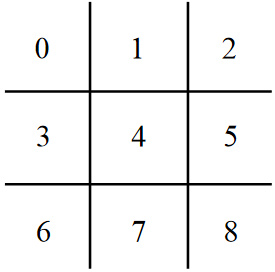
\includegraphics[width=3cm]{tictactoe_grid_linear.png}
  \end{center}
%
  Il metodo \texttt{toString()} dovr\`a descrivere il gioco con una
  stringa del tipo:
\begin{center}
\begin{verbatim}
X| |O
-----
X|O|O
-----
 | |X
\end{verbatim}
\end{center}
%
  Si noti che la classe \texttt{TicTacToe} \`e astratta perch\'e ha
  il metodo \texttt{isGameOver()} astratto. Tale metodo verr\`a implementato
  nelle sottoclassi.
\end{esercizio}

\begin{esercizio}~\textbf{[8 punti]}
  Si scriva la sottoclasse concreta \texttt{SimpleTicTacToe.java} di
  \texttt{TicTacToe.java} il cui metodo
  \texttt{isGameOver()} specifica che un gioco \`e finito quando
  non ci sono pi\`u caselle vuote.
  Si scriva la sottoclasse \texttt{RowsTicTacToe.java} di
  \texttt{SimpleTicTacToe.java} il cui metodo
  \texttt{isGameOver()} specifica che un gioco \`e finito quando
  non ci sono pi\`u caselle vuote oppure quando uno dei giocatori ha
  piazzato tre simboli uguali su una stessa riga o su una stessa colonna.
  Si scriva la sottoclasse \texttt{FullTicTacToe.java} di
  \texttt{RowsTicTacToe.java} il cui metodo
  \texttt{isGameOver()} specifica che un gioco \`e finito quando
  non ci sono pi\`u caselle vuote oppure quando uno dei giocatori ha
  piazzato tre simboli uguali su una stessa riga o su una stessa colonna
  o su una stessa diagonale.
\end{esercizio}

\begin{esercizio}~\textbf{[10 punti]}
  Si completi la classe \texttt{Main.java} in modo da creare un
  \texttt{FullTicTacToe} e fare giocare alternativamente
  Alessandra e poi Giovanni,
  leggendo ogni volta le coordinate $x$ e $y$ da tastiera, stampando
  il gioco dopo ogni mossa, finch\'e il gioco non risulta finito.
  Se una mossa genera un'eccezione, si stampi sul video il messaggio
  dell'eccezione e si torni a richiede una mossa corretta.
\end{esercizio}

\mbox{}\\

\emph{Se tutto \`e  corretto, un'esecuzione del \texttt{Main}
  dovrebbe rassomigliare a
  quanto riportato nel file di testo \texttt{risultato\_main.txt}.
}

\end{document}
